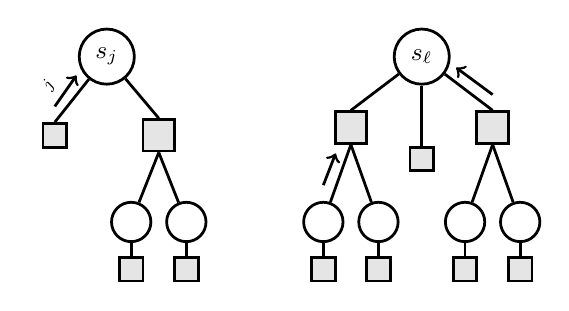
\begin{tikzpicture}
  [
  font=\small, line width=1pt, draw=black,
  check/.style={rectangle, minimum height=4mm, minimum width=4mm, draw=black, fill=gray!20},
  trivialcheck/.style={rectangle, minimum height=3mm, minimum width=3mm, draw=black, fill=gray!20},
  section/.style={circle, minimum size=7mm, draw=black},
  emptysection/.style={circle, minimum size=5mm, draw=black}
  ]

\node[section] (sp) at (0,0) {$s_{j}$};
\node[trivialcheck] (tp) at (-0.66,-1) {};
\node[check] (ap) at (0.66,-1) {};

\node[emptysection] (sp1) at (0.66-0.35,-0.9-1.2) {};
\node[trivialcheck] (tp1) at (0.66-0.35,-1.5-1.2) {}
    edge[-] (sp1);
\node[emptysection] (sp2) at (0.66+0.35,-0.9-1.2) {};
\node[trivialcheck] (tp2) at (0.66+0.35,-1.5-1.2) {}
    edge[-] (sp2);

\draw (sp) -- (tp.north);
\draw (sp) -- (ap.north);
\draw (sp1) -- (ap.south);
\draw (sp2) -- (ap.south);


\node[section] (sl) at (4,0) {$s_{\ell}$};
\node[trivialcheck] (tl) at (4,-1.3) {};
\node[check] (al1) at (4-0.9,-0.9) {};
\node[check] (al2) at (4+0.9,-0.9) {};

\node[emptysection] (sl11) at (3.1-0.35,-0.9-1.2) {};
\node[trivialcheck] (tl11) at (3.1-0.35,-1.5-1.2) {}
    edge[-] (sl11);
\node[emptysection] (sl12) at (3.1+0.35,-0.9-1.2) {};
\node[trivialcheck] (tl12) at (3.1+0.35,-1.5-1.2) {}
    edge[-] (sl12);

\node[emptysection] (sl21) at (4.9-0.35,-0.9-1.2) {};
\node[trivialcheck] (tl21) at (4.9-0.35,-1.5-1.2) {}
    edge[-] (sl21);
\node[emptysection] (sl22) at (4.9+0.35,-0.9-1.2) {};
\node[trivialcheck] (tl22) at (4.9+0.35,-1.5-1.2) {}
    edge[-] (sl22);

\draw (sl) -- (tl.north);
\draw (sl) -- (al1.north);
\draw (sl) -- (al2.north);
\draw (sl11) -- (al1.south);
\draw (sl12) -- (al1.south);
\draw (sl21) -- (al2.south);
\draw (sl22) -- (al2.south);


\draw[shorten <=0.22cm,<-] (sp.south west)++(0,0.2cm) -- node[above,rotate=58,xshift=-0.15cm] {$\lambdav_j$} ([yshift=0.2cm]tp.north);
\draw[shorten <=0.12cm,<-] (al1.south)++(-0.15cm,0) -- node[above,rotate=68,xshift=-0.1cm] {$\lambdav$} ([yshift=0.2cm]sl11.north);
\draw[shorten <=0.22cm,<-] (sl.south east)++(0,0.25cm) -- node[above,rotate=-45,xshift=0.15cm] {${\muv}$} ([yshift=0.2cm]al2.north);

\end{tikzpicture}
